\twocolumn[\begin{@twocolumnfalse}
	\chapter{Replacing the NABU Power Supply\hfill\difficulty{4}}
	The NABU Personal Computer was developed for the North-American market, and as such, was fitted with a 110-120V power supply unit (PSU). The following section explains how to replace the NABU power supply with a modern, universal power supply.
	Note that the replacement PSU referred to in this guide is the Mean Well RT-65B. Refer to the relevant manufacturer's documentation for connection details when using other makes or models.
	\vskip1em
\end{@twocolumnfalse}]
\section{Removing the NABU PSU}
\awesomebox[red]{2pt}{\faBolt}{red}{To prevent electric shock, you \textbf{must} disconnect your NABU Personal Computer from mains power before removing the system cover!}
\begin{enumerate}
	\item Remove the outer computer cover by undoing the screws on either side of your NABU system. This will expose the main system board (right) and power supply bay (left).
	\item Remove the cover over the power supply by undoing the two screws on the right-hand side and lifting the cover upwards.
	\item Disconnect the motherboard (a), mains (b), and ground (c) connectors, as shown in Figure \ref{fig:connectors} below.
	\begin{figure}[b!]
		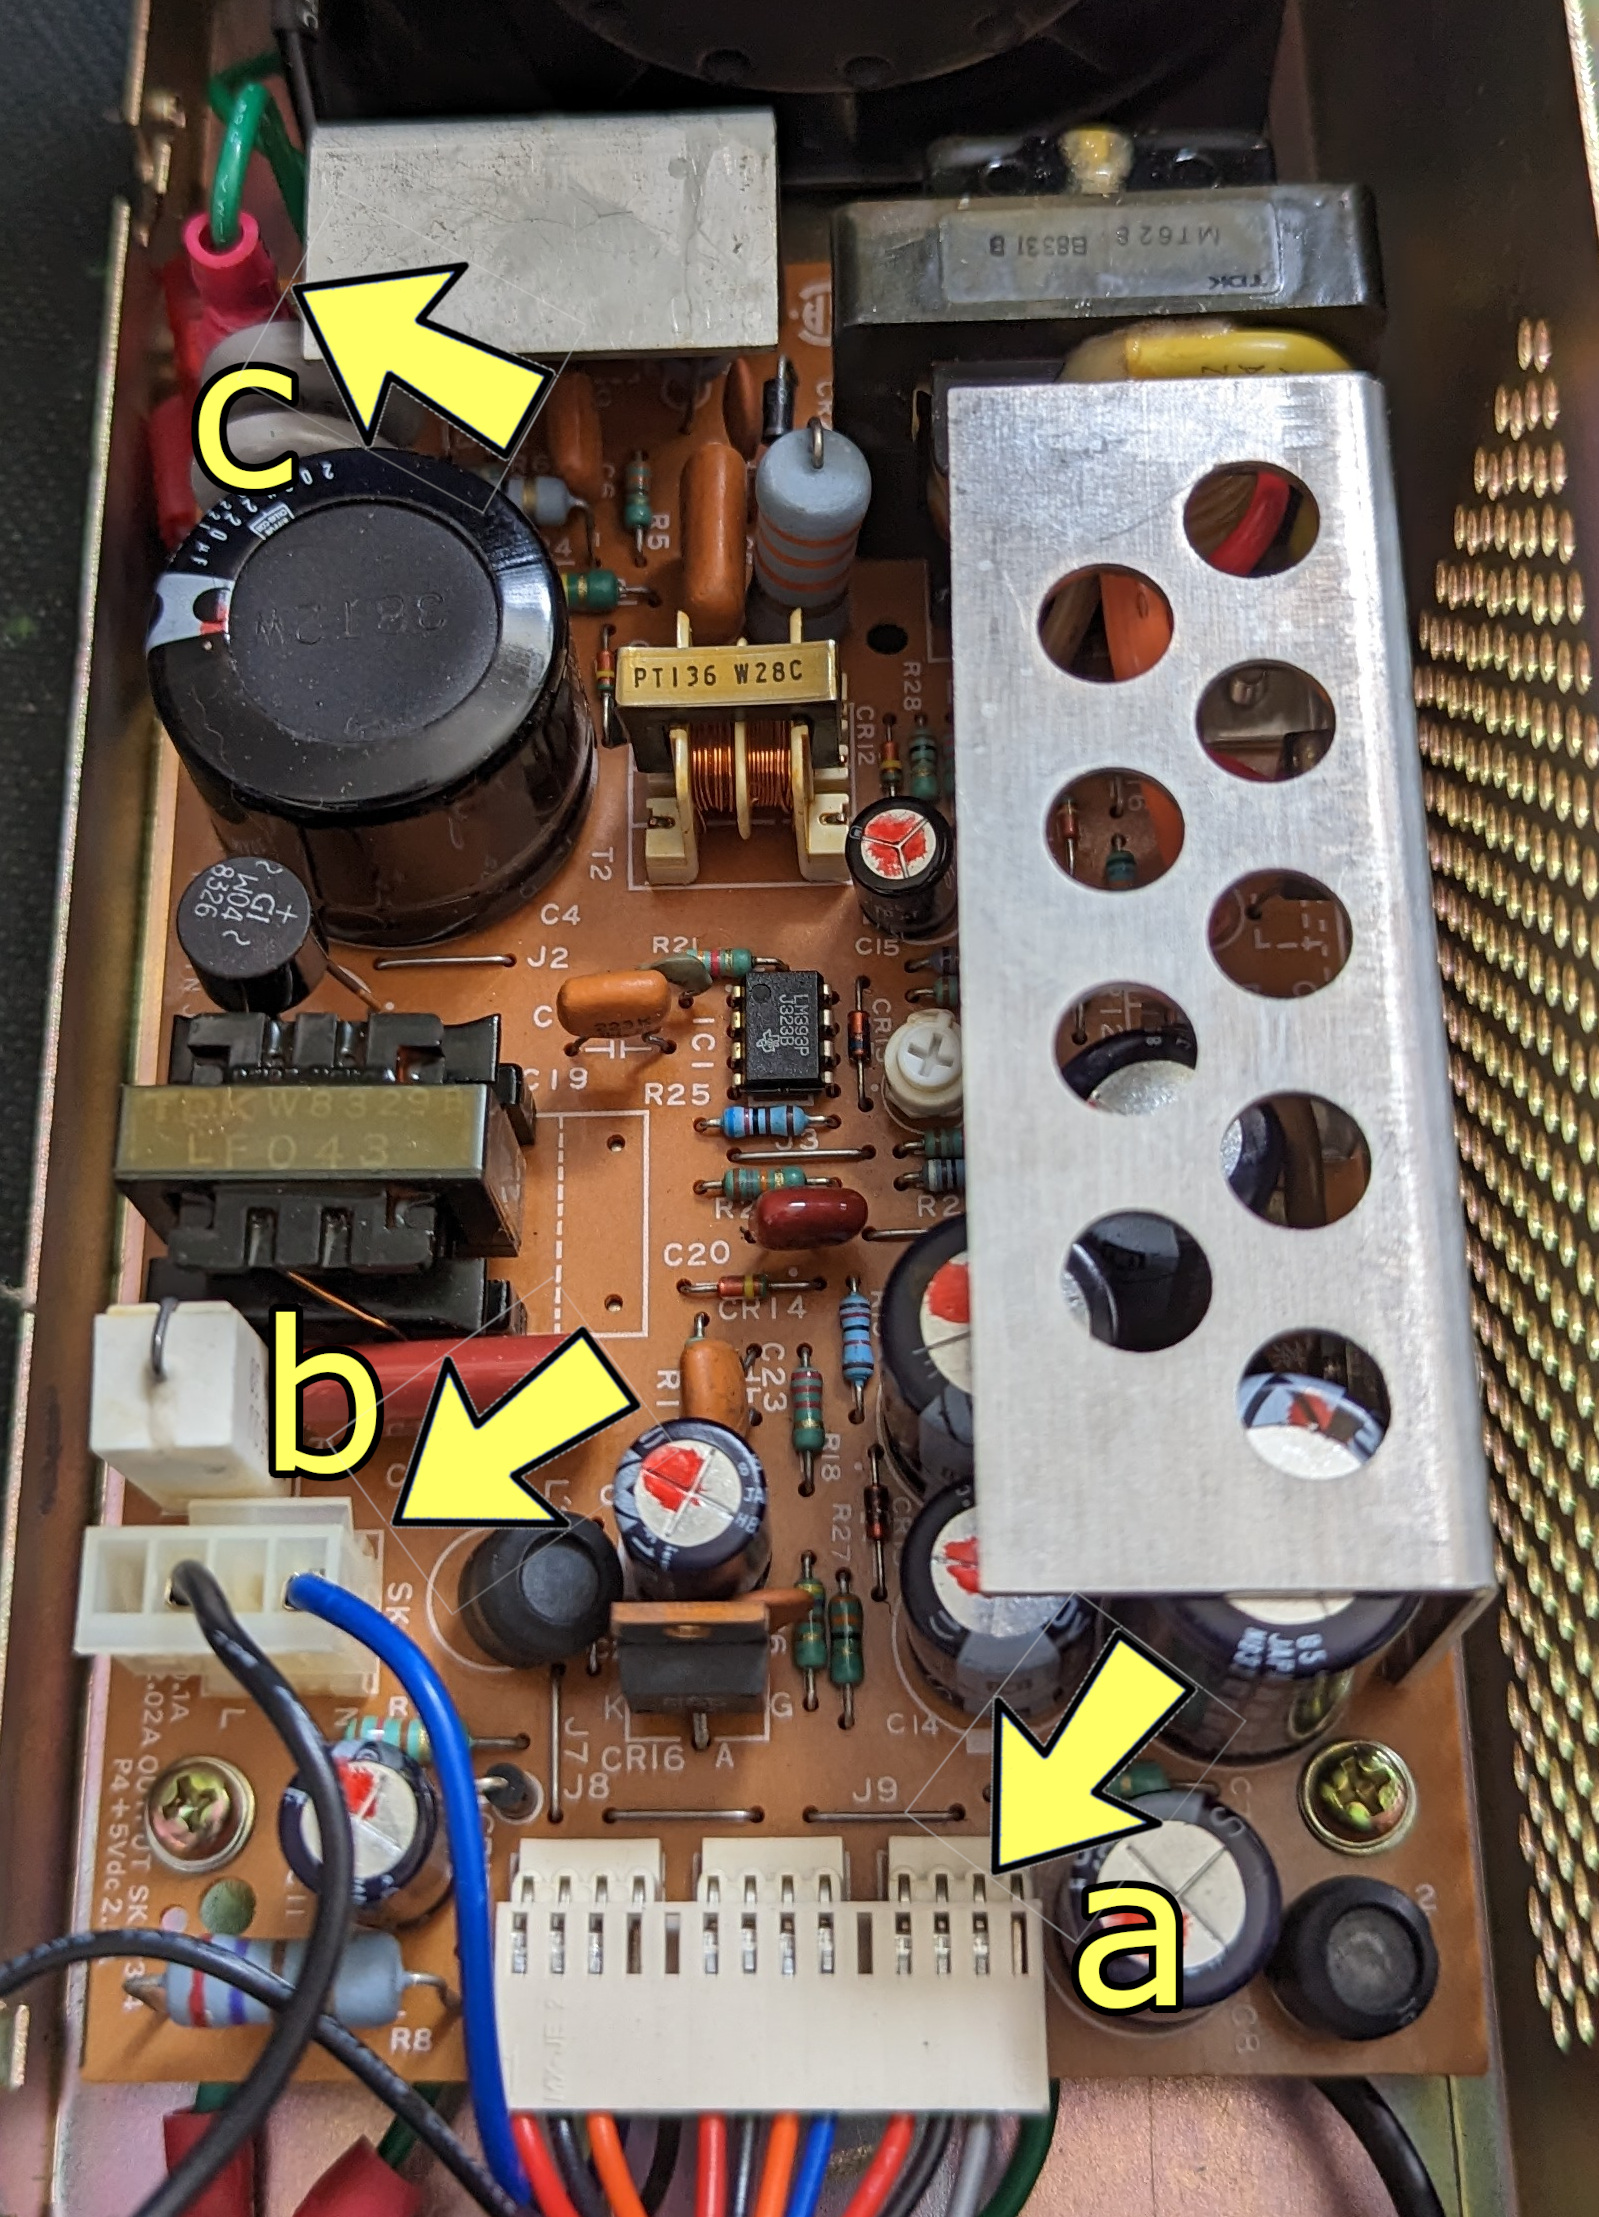
\includegraphics[width=\columnwidth]{images/psu-image-0.jpg}
		\caption{PSU connector positions.}
		\label{fig:connectors}
	\end{figure}
	\item Undo the 4 screws holding the PSU in place, and remove the PSU.
	\item Cut off both the motherboard (a) and mains (b) connectors as close as possible to each connector and strip a \textonequarter inch of insulation of the ends of all wires. Cut off the spade connector (c) and halve the length of the ground wire.
\end{enumerate}
\section{Replacing the NABU fan assembly}
\label{sec:fan-replacement}
As the fan fitted in the NABU power supply bay runs off 110-120V, it is no longer useful and should be removed. A suitable 80x80mm 12V or 5V fan may be fitted in its place.
\begin{enumerate}
	\item  To remove the fan, prise apart the crimp connector and cut the other lead near power button.
	\item Undo the 3 bolts which hold the assembly in place and remove the fan.
	\item Remove the remaining part of the fan power lead attached to the power button by gently removing the old heat shrink tubing and cutting the lead as close as possible to the terminal (see Figure \ref{fig:fan}). Then re-cover the terminal and remaining lead with a suitable length of new heat shrink tubing (as shown in Figure \ref{fig:tubing}).
	\item Remove the fan ground lead from the `ground post' by undoing the nut and lifting off the ring connector.
	\item Install the replacement fan using the bolts removed in the previous step, ensuring it is oriented such that air is sucked out of the NABU system. Guide the new fan leads towards the front of the system.
	\begin{figure}[h!]
		\begin{subfigure}[b]{\columnwidth}
			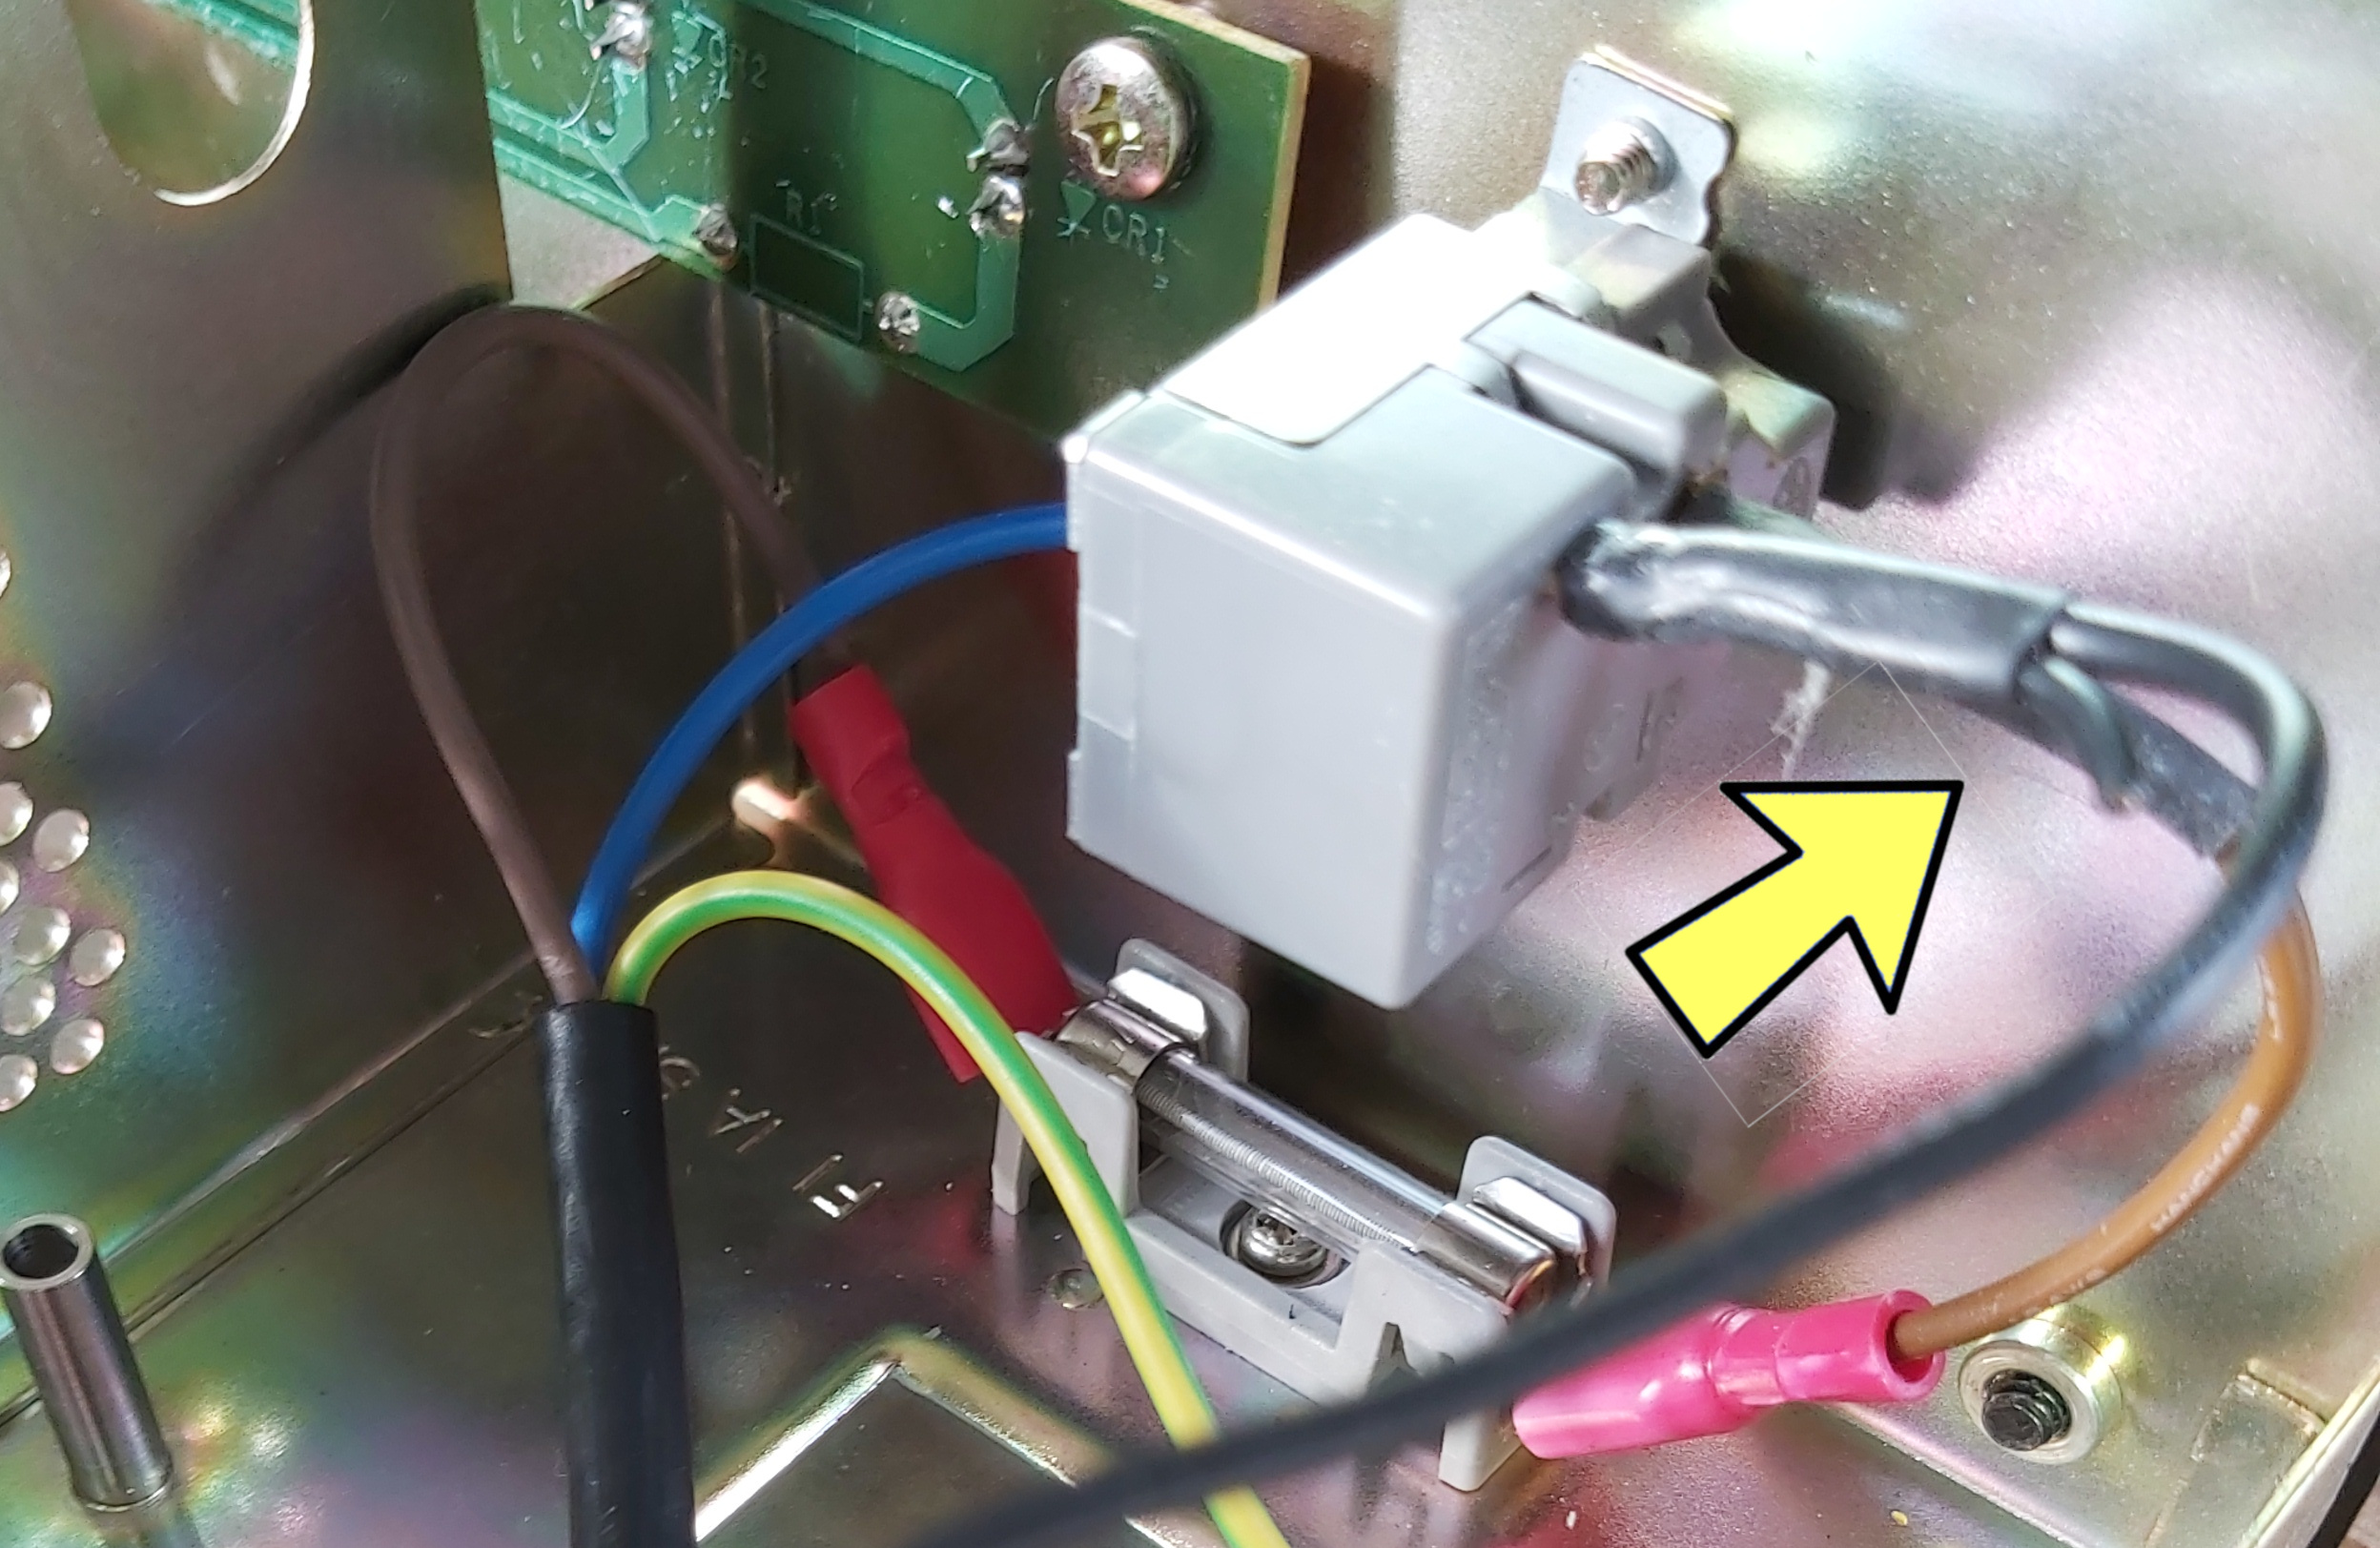
\includegraphics[width=\columnwidth]{images/psu-image-1a.jpg}
			\caption{Remove the remaining length of the fan power lead.}
			\label{fig:fan}
		\end{subfigure}
		\vskip1em
		\begin{subfigure}[b]{\columnwidth}
			%\end{figure}
			%\begin{figure}[t!]
			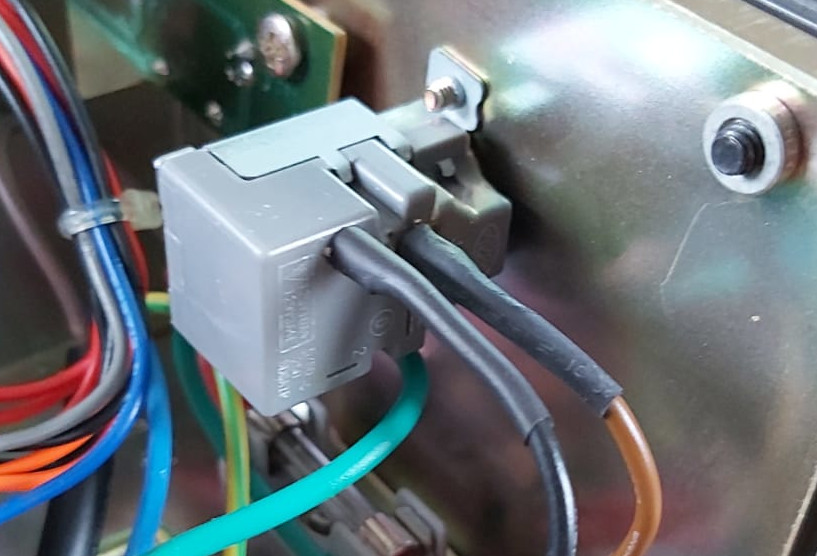
\includegraphics[width=\columnwidth]{images/psu-image-1b.jpg}
			\caption{Cover the power terminal with new heat shrink tubing.}
			\label{fig:tubing}
		\end{subfigure}
		\caption{Removing fan power lead.}
	\end{figure}
\end{enumerate}
\section{Replacing the mains cable}
The mains cable fitted to the NABU may be left in place and the Canada/US power plug replaced with a 3-pin domestic plug as appropriate. If the NABU cable is left in place, make note of the following colours and wire your domestic plug as shown in Table \ref{tbl:mains}.
\begin{center}
	\sffamily
	\begin{tblr}{
			colspec={|c|l|},
			hline{1,2,5},
			row{1} = {bg=gray4,fg=white,font=\bfseries},
			row{3} = {bg=gray9},
		}
		NABU lead & Function \\
		Green & Earth \\
		White & Neutral \\
		Black & Live \\
	\end{tblr}
	\taskLbl{tbl:mains}
	\taskTable{NABU mains lead details.}
\end{center}
Alternatively, the NABU mains cable can be replaced as following:
\begin{enumerate}
	\item Cut the NABU mains lead on the \textbf{inside} of the NABU system as close as possible to the strain relief bush grommet. Then pull the lead from the outside to free it from the grommet --- this may require some force and wriggling.
	\item Pass the new cable through the hole in the back of the case and secure it in place with the strain relief grommet recovered from the previous step. Allow enough length for the wires to comfortably reach the front of the NABU.
	\item Use a crimp tool to attach a ring connector to the mains Ground lead (green). Then attach a female spade connector to the Live lead (brown). Ensure that each connectors is securely attached to its lead to prevent poor contact.
	\item Firmly push the spade connector onto the fuse holder terminal. Loop the ring connector over the vertical `ground' post and secure it in place with a nut (as shown in Figure \ref{fig:new}). Note that the fuse itself does \textit{not} need to be replaced.
	\begin{figure}[h!]
		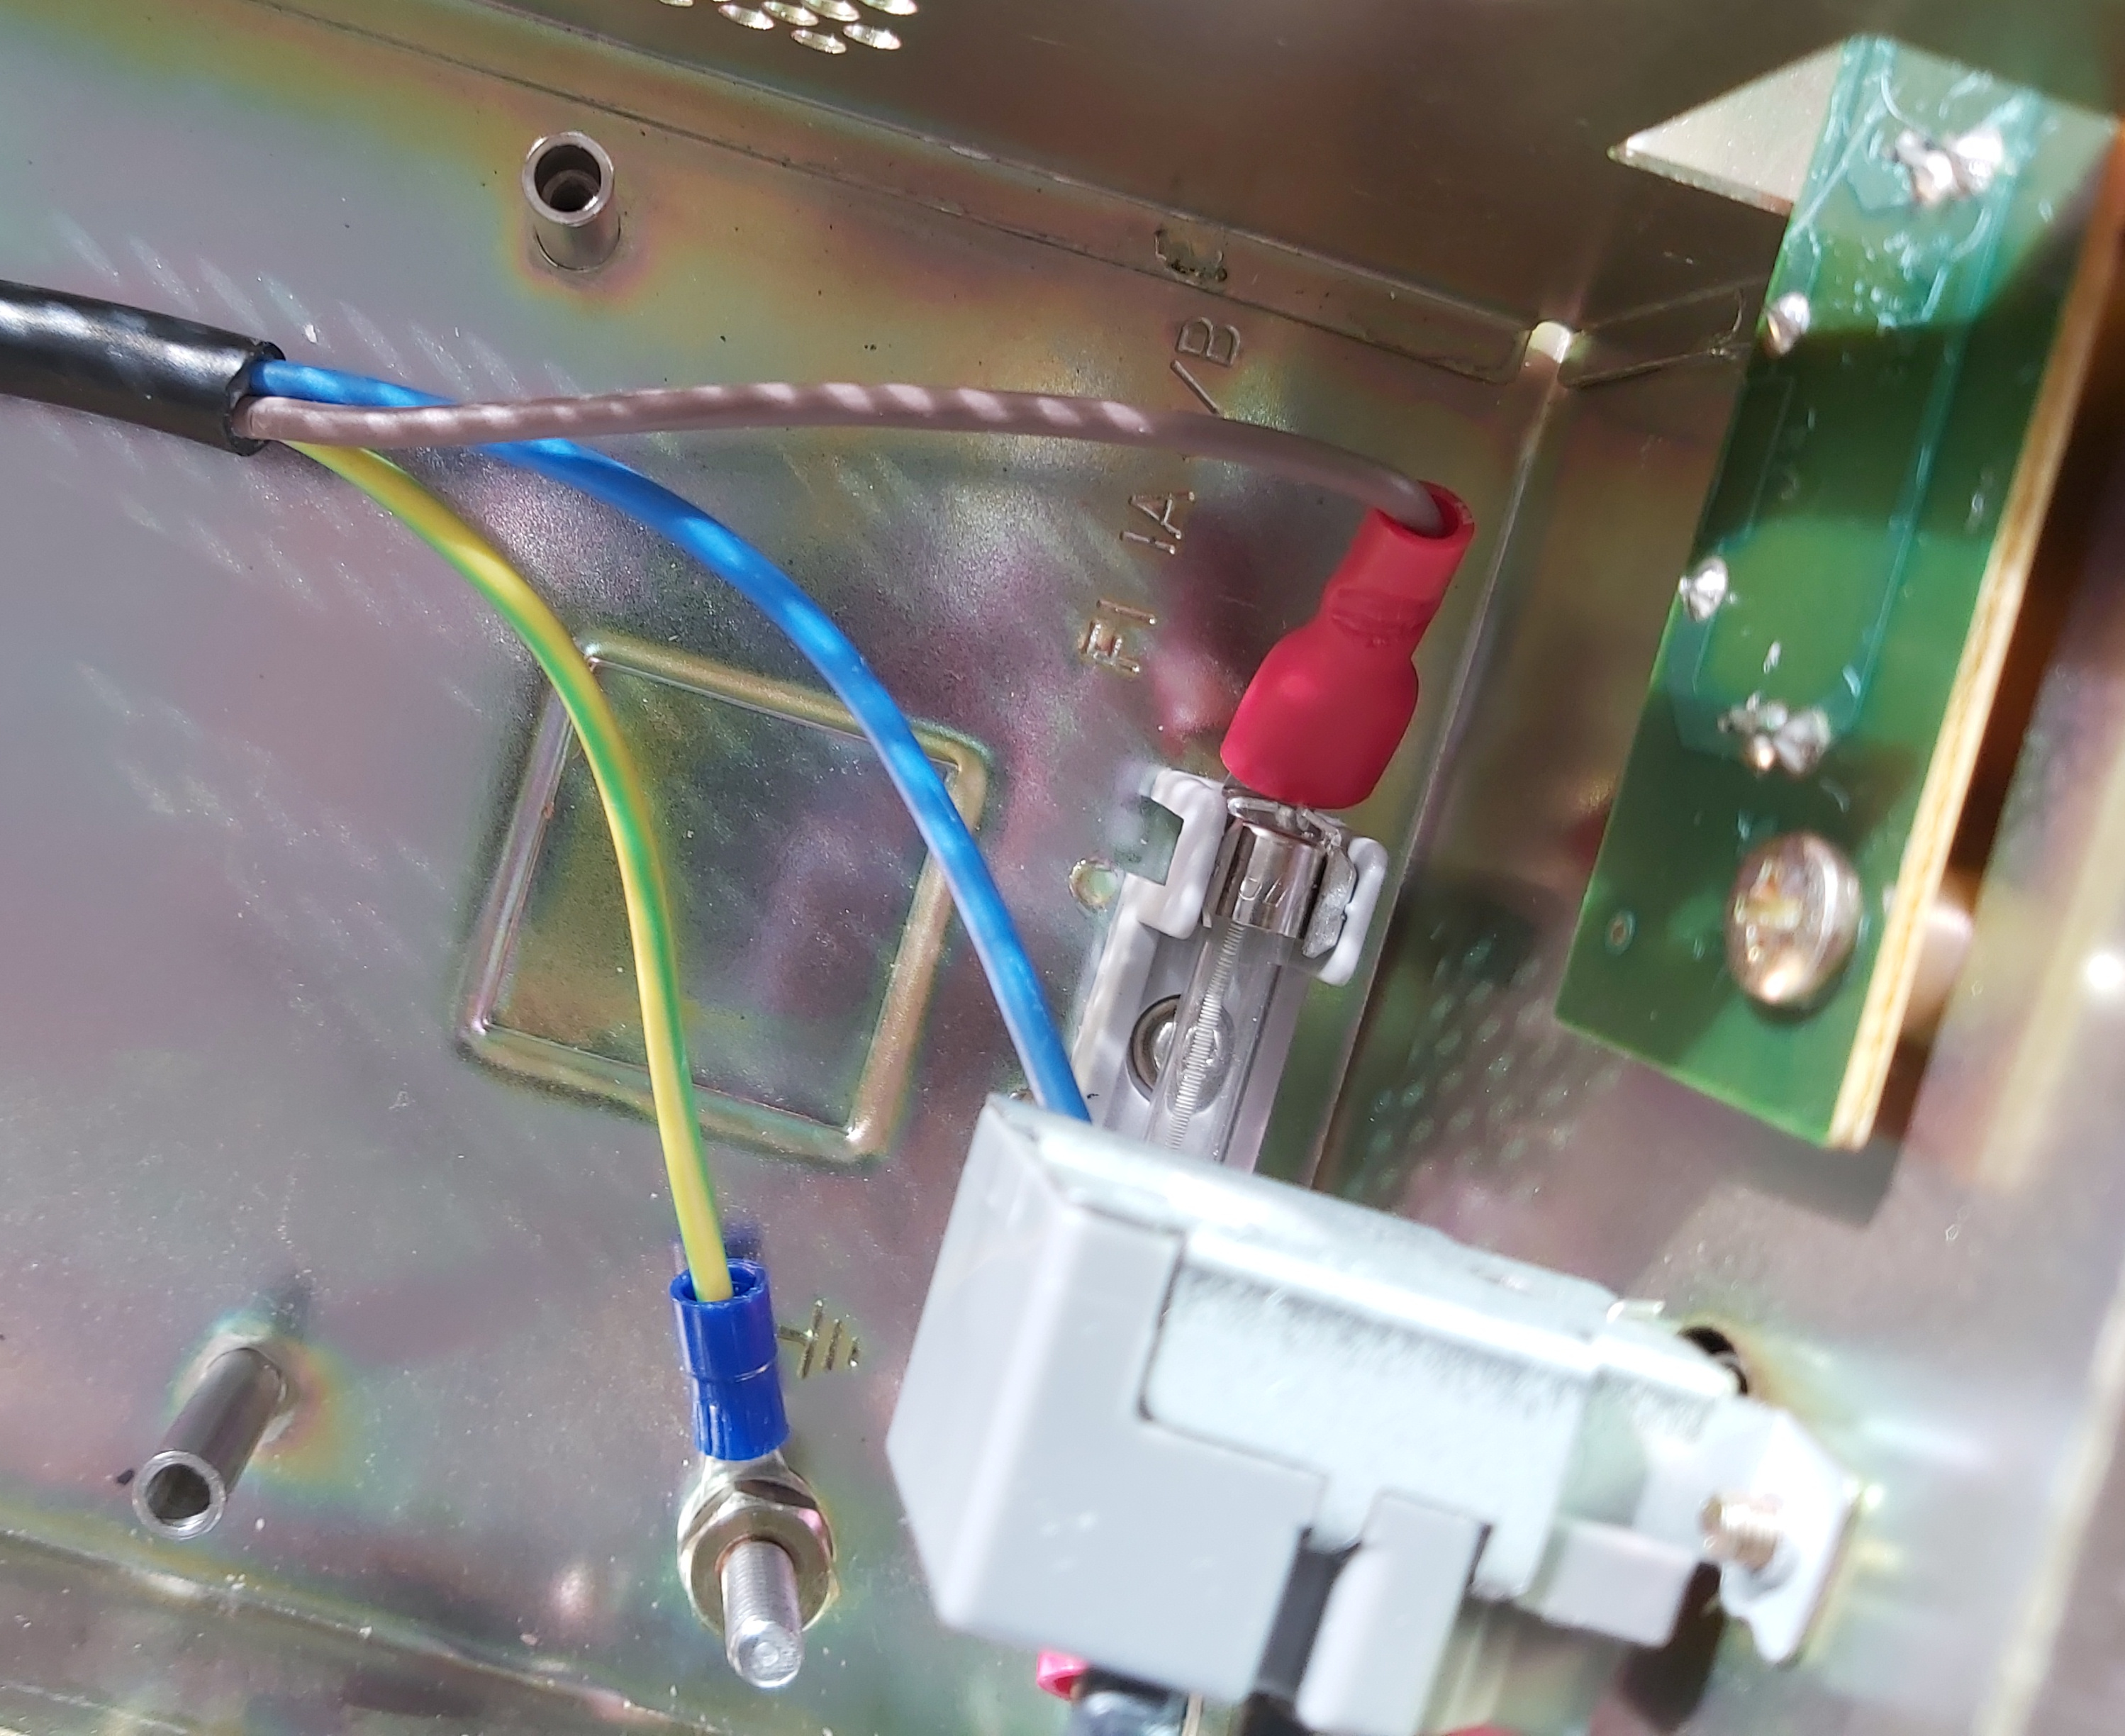
\includegraphics[width=\columnwidth]{images/psu-image-2.jpg}
		\caption{Connect the Ground (green) and Live (brown) wires.}
		\label{fig:new}
	\end{figure}
\end{enumerate}
\section{Installing the Mean Well PSU}
The NABU requires multiple voltage levels, as detailed in the following table. The first two columns show the Mean Well RT-65B PSU terminals and their corresponding levels. The remaining columns show the colour and number of NABU wires that must be connected to each terminal. For example, both the single grey wire and two orange wires need to be connected to the terminal labelled \bbox{+V2} on the PSU.
\begin{center}
	\sffamily
	\begin{tblr}{
			colspec={|c|c|c|c|},
			hline{1,2,7},
			row{1} = {bg=gray4,fg=white,font=\bfseries},
			row{3,4,6} = {bg=gray9},
			cell{3}{1} = {r=2}{c},
			cell{3}{2} = {r=2}{c}
		}
		RT-65B & Level & Colour & Wires \\
		\bbox{V3} & -12V & Blue & 1 \\
		\bbox{+V2} & +12V & Grey & 1 \\
		& & Orange & 2 \\
		\bbox{COM} & Ground & Black & 3 \\
		\bbox{+5V} & +5V & Red & 3 \\
	\end{tblr}
	\taskLbl{tbl:wiring}
	\taskTable{Motherboard wiring details.}
\end{center}
To install the replacement PSU:
\begin{enumerate}
	\item If the mains cable was replaced, reattach the short ground lead (green) to the ground post and fix it in place with a nut.
	\item Place the Mean Well PSU such that the mounting hole near the \bbox{+5V Adj} trimmer on the PSU is lined up with the front right-hand post in the NABU bay and fix it in place with a screw. Note that the other posts do not line up with the remaining PSU mounting holes, meaning the PSU is kept in place with only a single screw.
	\item Attach the mains wires as shown. Be careful not to mix up the mains wires with the wires connected to the NABU motherboard.
	\begin{center}
		\sffamily
		\begin{tblr}{
				colspec={|c|c|c|},
				hline{1,2,5},
				row{1} = {bg=gray4,fg=white,font=\bfseries},
				row{3} = {bg=gray9}
			}
			RT-65B & Level & Colour \\
			\bbox{~L~\null} & Live & Black \\
			\bbox{~N~\null} & Neutral & Blue \\
			\bbox{~$\Ground$~\null} & Ground & Green \\
		\end{tblr}
		\taskLbl{tbl:live}
		\taskTable{Mains wiring details.}
	\end{center}
	\item Connect the wires leading from the NABU motherboard, as shown in Table \ref{tbl:wiring} (above) and Figure \ref{fig:terminals}.
	\begin{figure}[h!]
		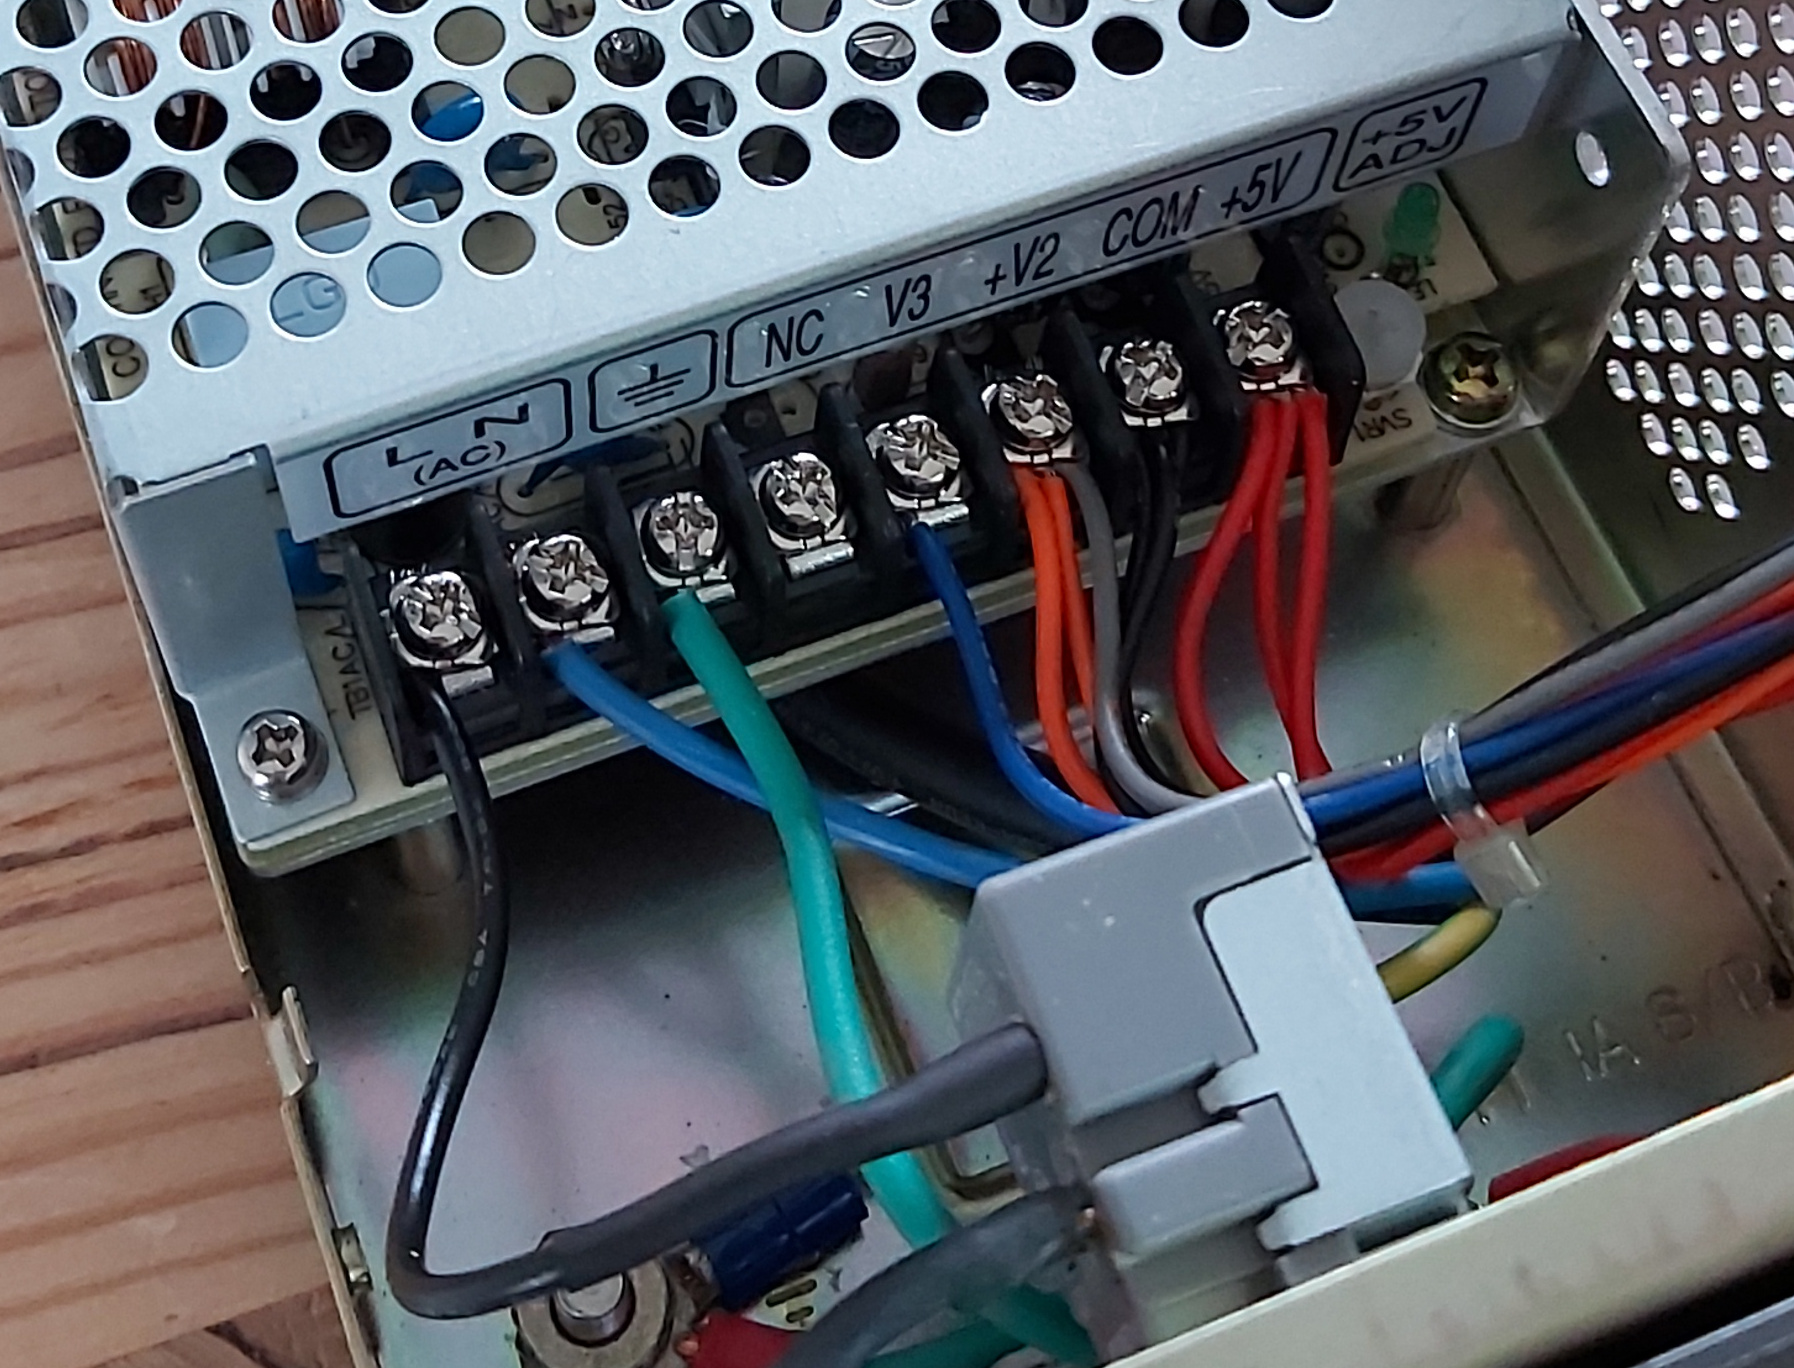
\includegraphics[width=\columnwidth]{images/psu-image-3.jpg}
		\caption{Connect all wires to the relevant PSU terminals.}
		\label{fig:terminals}
	\end{figure}
	\item Connect the new fan leads to the PSU \bbox{COM} and either \bbox{+5V} or \bbox{+V2} terminals as appropriate.
	\item Check there are no loose parts or unconnected wires --- any wires that remain unconnected \textbf{and are no longer required} must be trimmed and made safe, e.g. by covering them with electrical insulation tape or heat shrink tubing. Once you are satisfied that all wires are correctly and securely connected, replace the NABU PSU cover and fix in place with its 2 screws.
	\item Replace the NABU system cover, securing it with 4 screws.
\end{enumerate}
